\chapter{Development}\label{chap:development}
\section{Overview} 
This chapter presents some notes regarding project development, along with a description of how code is structured, tools and libraries used, and compiling pre-requisites and procedures.

\section{Project structure}
The whole project has been structured as a \emph{cmake}-based project, as this popular open source, cross-platform compiling tool provides the necessary flexbility to joint the different parts of the project. Thus, a single, top-level \emph{CMakeLists.txt} file (the \emph{cmake} project file) takes care of building all the components needed to build ther project. This top-level project file includes the nested \emph{CMakeFiles.txt} subproject files belonging to the kernel module, the C/C++ library, the unit tests, and the CLI userspace tools.

Put short, the project is internally structured in 3 parts:
\begin{itemize}
	\item The kernel module
	\item The C/C++ library (including unit tests)
	\item The CLI tools
\end{itemize}


\subsection{Kernel module}
Kernel module (\emph{jsmapperdev}) code is located under \emph{src/linux/drivers/input} folder, following a layout that mimics that of Linux kernel source. 

As \emph{cmake} doesn't support (as of today) a native way to compile kernel modules, an special set of custom commands are used inside the \emph{CMakeFiles.txt} project file for the module. These commands end up by calling the native Linux build system (\emph{Kbuild}) for kernel modules, which relies on scripts located under \emph{/lib/modules/<kernel version>/build/} folder.

The kernel module is implemented by this set of source files:
\begin{itemize}
	\item \textbf{jsmapper\_api.h}: contains API definitions, such as IOCTL codes and parameter structures. This file is the only one designed to be included both from kernel project and from userspace tools.
	\item \textbf{jsmapper\_main.c}: contains the module frontend, consisting in the basic code needed to implement a kernel module, the input event filter callbacks, etc...
	\item \textbf{jsmapper\_core.c}: contains the mapping core, this is, the data structures containing the mapping data which get associated to every \emph{jsmap} device node.
	\item \textbf{jsmapper\_evgen.c}: contains the code for the virtual event generator
	\item \textbf{Kbuild}: contains the instructions for the Linux kernel build system (\emph{Kbuild}) needed to build the module.
\end{itemize}
 
On install, the kernel module will be copied under \emph{/lib/modules/<kernel version>/kernel/drivers/input/}.

\subsubsection{Event filtering}
Event filtering on the target hardware device is provided by the \emph{jsmapper\_filter()} function in \emph{jsmapper\_main.c} module. 

This function is called by the kernel everytime an event is generated from the device: the function then checks if the source event is mapped to any action, and takes the appropiate steps to launch it. Depending on the source element type, the steps performed will be different:
\begin{itemize}
	\item For buttons, it will \emph{start} the action when the button is being pressed, and \emph{stop} it if the button is being reelased.
	\item For axes, it will \emph{start} the action when the axis is moved into the band the action is mapped to, and it will \emph{stop} the action when the axis is moved outside of the band. 
\end{itemize}

Finally, it returns a boolean value to the kernel indicating if the source event must be filtered out, or else it must be let go its way to the other attached event handlers.


\subsubsection{Event generation}
Simulated events get injected into the input core by calling the kernel-provided function \emph{input\_event()}, which is the function called also from the ``real'' device drivers when they notify changes in device controls upon user interaction.

For simple keystrokes and mouse button clicks, the referred function is called directly from the context of the event filtering function mentioned above. 

For complex actions, different mechanisms are used to avoid blocking the filtering thread which is being invoked from an IRQ context, as it provides some restrictions: for instance, from IRQ code the \emph{wait()} call (used to wait some milliseconds) can't be used, as the scheduler is not accessible from that point and thus no other thread can be scheduled.
\begin{itemize}
 \item Macros are sent using a \emph{workqueue} item: this is a low-level mechanism provided by Linux kernel which allows to ''queue`` some action to be done into a workqueue, serviced by a background thread that gets activated when some job to be done is posted. The service thread doesn't run into IRQ context but normal process context, so it can safely use \emph{wait()} calls to keep the cadence, etc...
 \item Mouse moving actions are implemented using a \emph{kernel thread}, which keeps sending axis movement events in the background for as long as the action is kept ``active. As ''workqueue`` service thread, this thread runs in normal ''process`` context, so it doesn't have the restrictions of IRQ context.
\end{itemize}


\subsection{C/C++ Library}
The C/C++ library (named \emph{jsmapper}) is located under \emph{src/lib/jsmapper} folder. It provides C++ wrapper classes useful to programatically interact with the driver, without the need of dealing with IOCTL calls. It also provides higher level functions, such as profile XML serialization.

All library classes are located inside \emph{jsmapper} namespace, to avoid name collisions. On install, the library files will get installed under \emph{\$PREFIX/lib/} folder.

Figure \ref{fig:dev_classes} displays the classes provided by the library, along with their inheritance and relationship diagram.

As a side note, the CLI tools are built using the library instead of the IOCTL API directly.

\begin{figure}[tp]
\centering
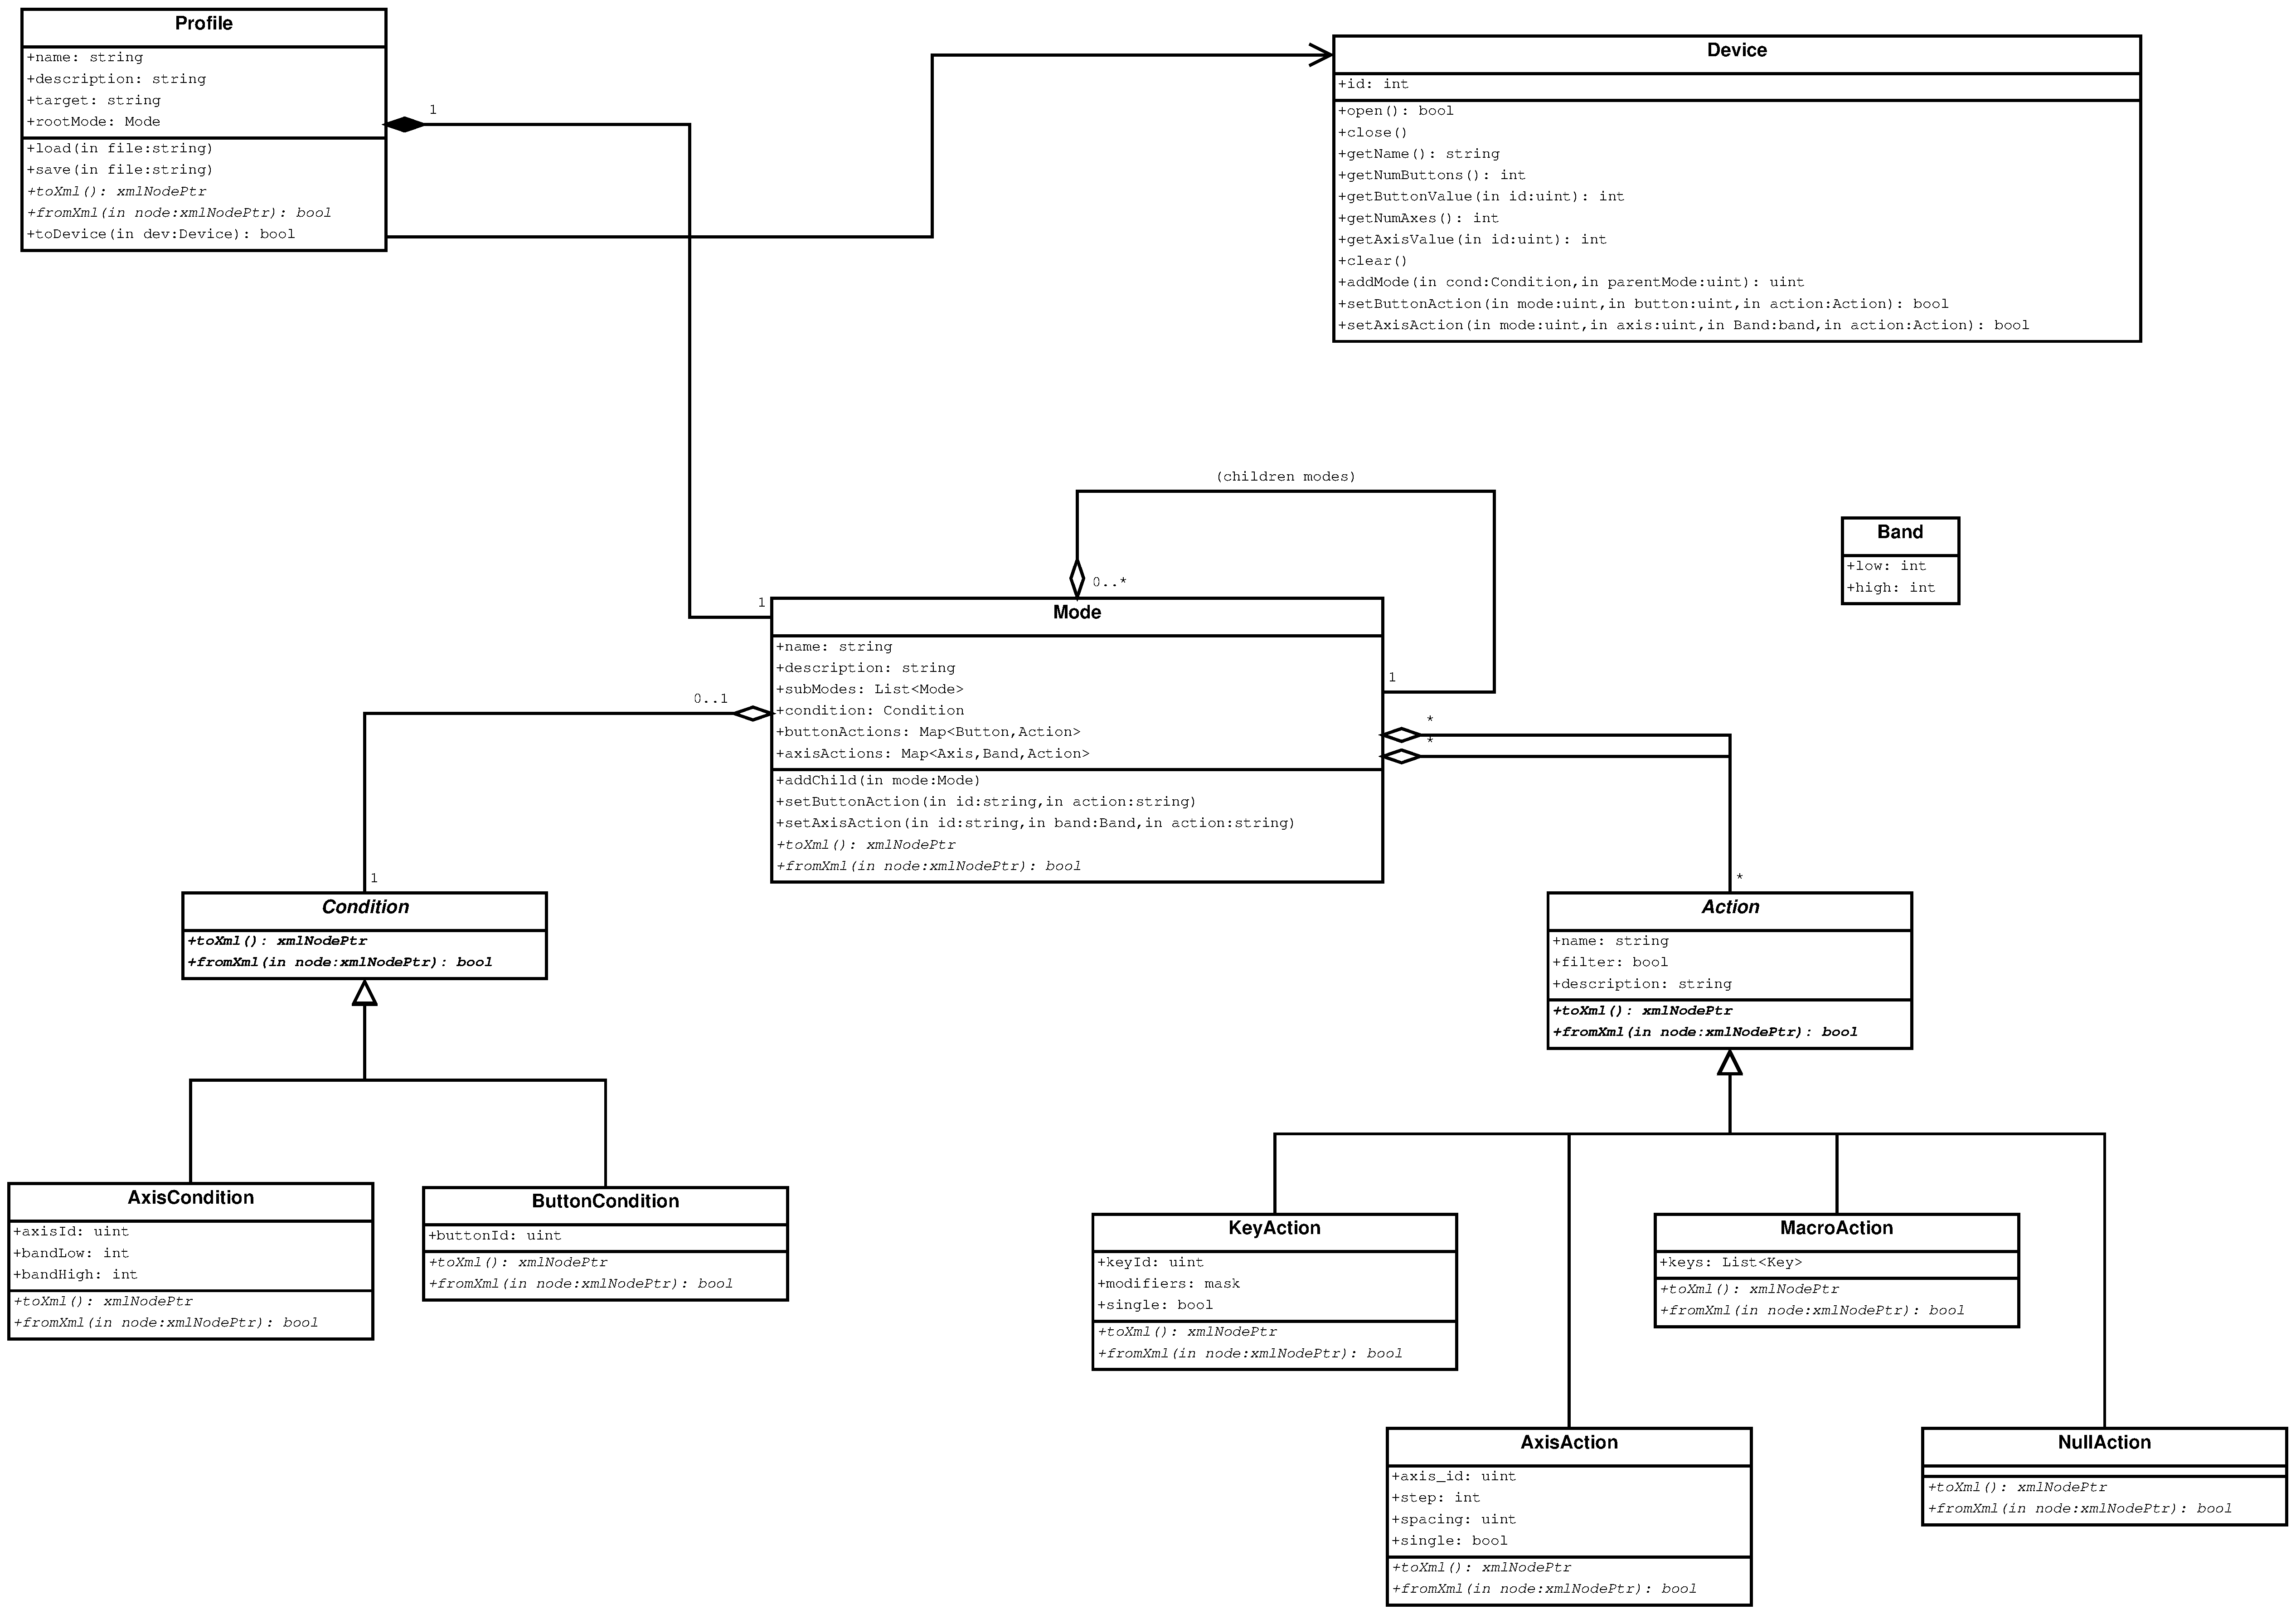
\includegraphics[totalheight=0.75\textheight, angle=90]{classes}
\caption{Class Diagram}
\label{fig:dev_classes}
\end{figure}


\subsection{Unit tests}
A number of unit tests are included along the library, to test the correct behaviour of the classes provided. These tests are located under \emph{src/test/} subfolder, and they are built around \emph{gtest}, this is, the ``Google C++ Test Framework'', whose code is also embedded with the project.

Unit tests can be invoked by issuing \emph{make test} command on the build directory (see section~\ref{section:compiling} below). When installing, the executable test binaries will get copied to \emph{\$PREFIX/bin/}, along with CLI tools.


\subsection{CLI tools}
The CLI tools are located under \emph{src/bin/} subfolder. Two executable tools are provided:
\begin{itemize}
  \item \textbf{jsmapper-ctrl}: basic CLI tool used to load profiles into the driver, clearing the state, etc...
  \item \textbf{jsmapper-device}: helper tool used to write ``device maps'' for the attached device
\end{itemize}

When installing, the executable binaries will get copied to \emph{\$PREFIX/bin/} folder.


\subsection{Documentation}
The project code is documented using standard \emph{Doxygen} tags. This applies to both the kernel driver code, the C/C++ library and the CLI tools. A Doxygen configuration file is provided (\emph{doxy.cfg} inside ``doc'' folder) that can be used to generate the HTML documentation in the following way:
\begin{lstlisting}[language=bash,caption={Generating HTML documentation},label={lst:jsmapper_doxygen}]
$ doxygen doxy.cfg
\end{lstlisting}

The HTML documentation will be generated under the ``html'' subfolder.


\section{Compiling the project}\label{section:compiling}
\subsection{Pre-requisites}
The following components must be installed in the system before attempting to compile the project:
\begin{itemize}
	\item \emph{Git} (for code checkout)
	\item \emph{C/C++ compiler} (gcc, i.e.)
	\item \emph{cmake} (the whole project is cmake-based)
	\item \emph{kernel headers} (to build the kernel module)
	\item \emph{libncurses5} (development package)
	\item \emph{libxml2} (development package)
\end{itemize}

\subsection{Code checkout}
JSMapper code is currently hosted in Assembla, and can be accessed by cloning the remote Git repository into the compiling machine:
\begin{lstlisting}[language=bash,caption={Checking out the code},label={lst:jsmapper_checkout}]
$ git clone https://git.assembla.com/jsmapper.git
\end{lstlisting}

This will clone the project into a subdirectory named ``jsmapper''. The code itself is inside the ``src'' subfolder.

\subsection{Compiling and installing}
As with any CMake-based project, out-of-the-tree compiling is the preferred way to proceed, so a ``build'' directory must be created first. Then cmake must be invoked from within the build directory to create the makefiles, and then finally we can go with the usual \emph{``make \&\& (sudo) make install''} sequence.

From the shell:
\begin{lstlisting}[language=bash,caption={Compiling the project},label={lst:jsmapper_build}]
$ mkdir build
$ cd build
$ cmake <path-to-jsmapper>/src 
$ make
$ sudo make install
$ sudo depmod -a
$ sudo ldconfig 
$ sudo modprobe jsmapperdev
\end{lstlisting}

This will compile the project and install the binaries into the appropiate system locations. The (\emph{ldconfig}) step might be necessary depending on the system, in order for the installed binaries to find the library.

If no problems are found, then the last step should have loaded the kernel module succesfully, which can be verified by calling \emph{lsmod} and checking that \emph{jsmapperdev} is listed. In case of error, \emph{dmesg} it's usually a valuable source of information.


\section{Tools used}
The following software tools has been used for the project development:
\begin{itemize}
	\item \emph{QtCreator}, as the main IDE tools
	\item \emph{GNU C/C++ compiler}
	\item \emph{openSUSE}, \emph{Fedora} and \emph{Ubuntu} OS, running on the various development and testing PC computers
	\item \emph{LaTeX} and \emph{Kile} (KDE frontend for LaTeX) for this report
	\item \emph{GanttProject} for the Gantt diagram and task list
	\item \emph{Assembla}, as the hosting platform
\end{itemize}

In addition to the computers used for development, the following two game devices has been used for testing:
\begin{itemize}
	\item \emph{Saitek X-45 HOTAS}, a very popular device among flight simulator enthusiasts.
	\item \emph{Logitech Wingman Extreme}, an entry-level joystick
	\item \emph{Trust FF380 Force Feedback Racemaster}, a wheel drive and pedals combo used for car racing simulators.
\end{itemize}

The JSMapper features has been tested against the following games:
\begin{itemize}
	\item \emph{FlightGear}, a very popular open source flight simulator software, running natively on Linux
	\item \emph{Trackmania}, a Windows car racing simulator running under Wine on Linux.
\end{itemize}
